% begin module arc-length-ex1
\begin{frame}
\begin{example}[Example 1, p. 562]
Find the length of the arc of $y^2 = x^3$ between $(1,1)$ and $(4,8)$.
\begin{columns}[c]
\column{.3\textwidth}
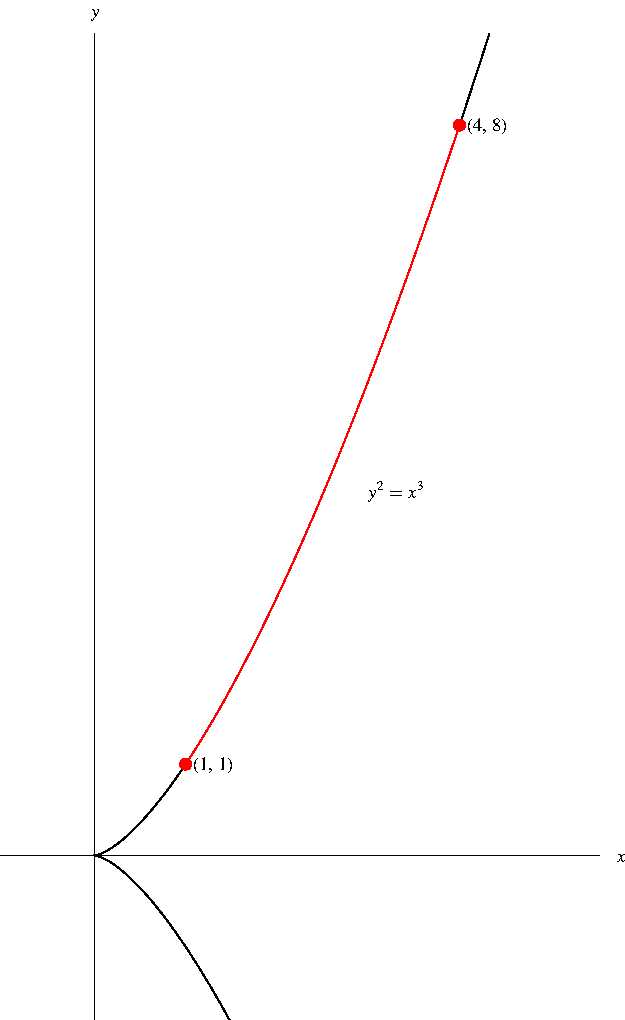
\includegraphics[height=6cm]{arc-length/pictures/09-01-ex1.pdf}%
\column{.7\textwidth}
\begin{itemize}
\item<2->  For the top half of the curve we have:
\item<2->  \alert<handout:0| 3-4>{$y = \uncover<4->{x^{3/2}}$} and  \alert<handout:0| 5-6,8>{$y' = \uncover<6->{\frac{3}{2}x^{1/2}}$}.
\item<9->  \alert<handout:0| 10-11>{$u = \uncover<11->{1 + \frac{9}{4}x}$} and  \alert<handout:0| 12-13>{$\diff u = \uncover<13->{\frac{9}{4}\diff x}$}.
\item<9-| alert@14-15>  When $x = 1$, $u = \uncover<15->{\frac{13}{4}}$.
\item<9-| alert@16-17>  When $x = 4$, $u = \uncover<17->{10}$.
\end{itemize}
\begin{eqnarray*}
\uncover<7->{%
L % 
}%
& \uncover<7->{ = } &%
\uncover<7->{%
\int_1^4 \sqrt{1+\left( \alert<handout:0| 8>{y'} \right)^2}\diff x%
}\\%
& \uncover<8->{ = } &%
\uncover<8->{%
\int_{\alert<handout:0| 14-15>{1}}^{\alert<handout:0| 16-17>{4}} \sqrt{\alert<handout:0| 11>{1+} \alert<handout:0| 8,11>{\frac{9}{4}x} }\ \alert<handout:0| 12-13>{\diff x}%
} \uncover<9->{ = } \uncover<9->{%
\int_{\alert<handout:0| 14-15>{\uncover<15->{13/4}}}^{\alert<handout:0| 16-17>{\uncover<17->{10}}} \alert<handout:0| 12-13>{\uncover<13->{\frac{4}{9}}}\uncover<11->{\sqrt{\alert<handout:0| 10-11>{u}}}\ \alert<handout:0| 12-13>{\uncover<13->{\diff u}}%
}\\%
& \uncover<18->{ = } &%
\uncover<18->{%
\frac{4}{9}\left[ \frac{2}{3} u^{3/2}\right]_{13/4}^{10}%
} \uncover<19->{ = } \uncover<19->{%
\frac{8}{27}\left( 10^{3/2} - \left( \frac{13}{4}\right)^{3/2}\right)%
}\\%
\end{eqnarray*}
\end{columns}
\end{example}
\end{frame}
% end module arc-length-ex1
